\chapter{Química verde y procesos industriales}\label{ch:b3:green-industrial}

El ibuprofeno se fabricaba antes en seis etapas que desechaban más masa de la que
conservaban: sales de aluminio, cloruro de sodio, etanol, amoníaco y ácido acético salían
de la planta por cada kilogramo de fármaco. Desde 1992, una ruta catalítica de tres etapas
convierte en producto la mayoría de los átomos que usa, y su único
subproducto, el ácido acético, se recupera y se vende. Este capítulo pone cifras a
esas comparaciones: \omterm{def:b3:green-industrial:atom-economy}{economía atómica}, \omterm{def:b3:green-industrial:e-factor}{factores E} e \omterm{def:b3:green-industrial:pmi}{intensidad de masa del proceso}; examina después
los disolventes, la energía y el \omterm{def:b3:green-industrial:lca}{análisis del ciclo de vida}, cómo se hicieron más limpios algunos de los
mayores procesos químicos, y lo que cambian las \omterm{def:b3:green-industrial:feedstock}{materias primas renovables} y las
\omterm{def:b3:complex-kinetics:enzyme}{enzimas}.

\begin{recall}
El volumen escolar introdujo la \omterm{def:b3:green-industrial:atom-economy}{economía atómica} y la \omterm{def:b3:green-industrial:green-chemistry}{química verde}; el volumen del primer
año, los rendimientos; el volumen del segundo año, los reactores, la conversión, la selectividad, el tiempo de
residencia, la conversión por paso, el reciclado y la purga, el aumento adiabático de temperatura,
los electrolizadores y las pilas de combustible. Los \cref{ch:b3:surfaces-catalysis} y
\cref{ch:b3:homogeneous-catalysis} trataron la catálisis, y
el \cref{ch:b3:total-synthesis}, las medidas de una ruta de síntesis.
\end{recall}

\begin{omfigure}
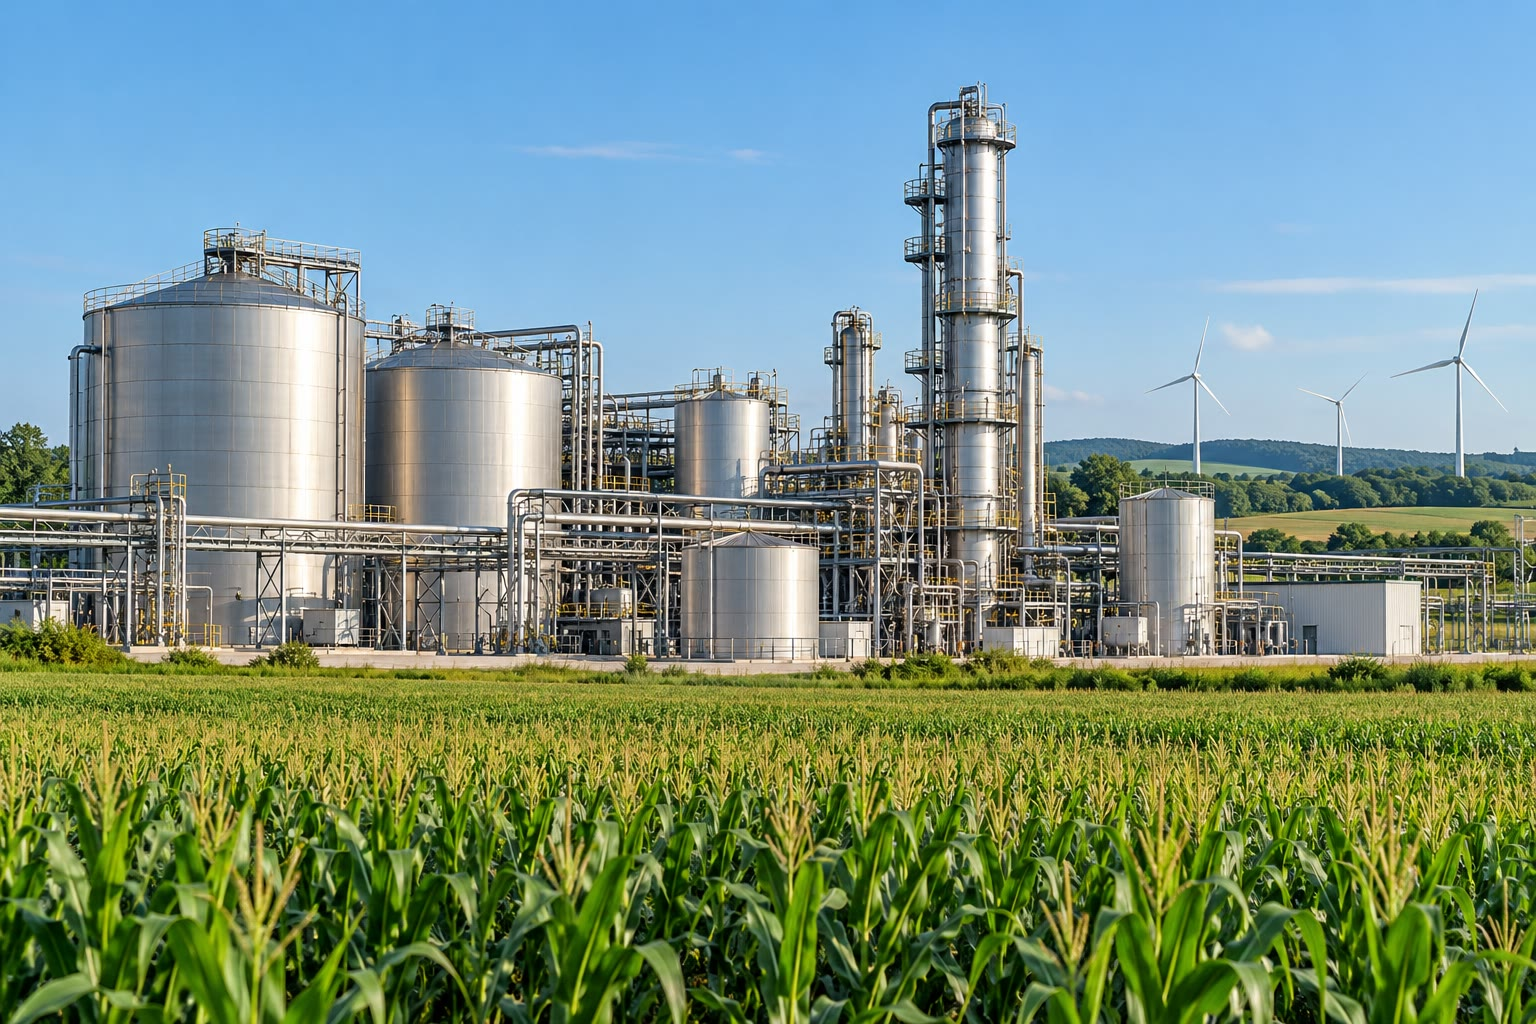
\includegraphics[width=0.58\linewidth]{images/book4/ai/b3-31-biorefinery.jpg}

{\small Una biorrefinería: tanques de fermentación y una columna de destilación que convierten
cultivos y residuos en combustibles y en productos químicos plataforma.}
\end{omfigure}

\section{Medir lo verde}

\begin{definition}[Química verde]\label{def:b3:green-industrial:green-chemistry}
La \emph{química verde}\index{quimica verde@química verde} es el diseño de productos y procesos
químicos que reducen o eliminan el uso y la generación de
sustancias peligrosas, resumido en doce principios: prevenir los residuos, maximizar la
\omterm{def:b3:green-industrial:atom-economy}{economía atómica}, usar y fabricar sustancias menos peligrosas, diseñar productos más seguros,
usar disolventes más seguros, ahorrar energía, usar \omterm{def:b3:green-industrial:feedstock}{materias primas renovables}, evitar derivados
innecesarios, preferir los catalizadores a los reactivos estequiométricos, diseñar para la
degradación, controlar en tiempo real y elegir una química intrínsecamente más segura.
\end{definition}

\begin{definition}[Economía atómica]\label{def:b3:green-industrial:atom-economy}
La \emph{economía atómica}\index{economia atomica@economía atómica} de una reacción es la masa molar del
producto deseado dividida por la suma de las masas molares de todos los
reactivos de la ecuación ajustada, expresada en porcentaje.
\end{definition}

\begin{proposition}[Economía atómica según el tipo de reacción]\label{prop:b3:green-industrial:ae-classes}
Las adiciones y las transposiciones tienen una \omterm{def:b3:green-industrial:atom-economy}{economía atómica} del 100\,\%; las sustituciones y las
eliminaciones, menos.
\end{proposition}

\begin{proof}
En una adición, $\mathrm{A} + \mathrm{B} \to \mathrm{AB}$, o en una transposición, $\mathrm{A} \to \mathrm{A'}$, el único producto contiene todos los
átomos de los reactivos, de modo que su masa molar es igual a la suma de las de estos. Una
sustitución, $\mathrm{A{-}X} + \mathrm{Y} \to \mathrm{A{-}Y} + \mathrm{X}$, o una eliminación, $\mathrm{A} \to \mathrm{B} + \mathrm{C}$, produce un
segundo producto que se lleva masa.
\end{proof}

\begin{definition}[Factor E]\label{def:b3:green-industrial:e-factor}
El \emph{factor E}\index{factor E} de un proceso es la masa de residuos por masa de
producto. En el factor E completo, todas las entradas que no acaban en el producto cuentan como
residuos, incluidos los disolventes y el agua; el factor E simple deja fuera los disolventes y el
agua.
\end{definition}

\begin{definition}[Intensidad de masa del proceso]\label{def:b3:green-industrial:pmi}
La \emph{intensidad de masa del proceso}\index{intensidad de masa del proceso} (PMI) es la
masa total de materiales introducidos en un proceso (reactivos, reactivos auxiliares, disolventes,
agua) por masa de producto.
\end{definition}

\begin{proposition}[PMI y factor E]\label{prop:b3:green-industrial:pmi-e}
Para un mismo límite, $\mathrm{PMI} = E + 1$, donde $E$ es el \omterm{def:b3:green-industrial:e-factor}{factor E} completo.
\end{proposition}

\begin{proof}
Por la conservación de la masa, todo lo que entra sale como producto o como residuo:
$m_{\mathrm{ent}} = m_{\mathrm{producto}} + m_{\mathrm{residuo}}$. Dividiendo por $m_{\mathrm{producto}}$ se obtiene $\mathrm{PMI} = 1 + E$.
\end{proof}

\begin{definition}[Eficiencia másica de reacción]\label{def:b3:green-industrial:rme}
La \emph{eficiencia másica de reacción}\index{eficiencia masica de reaccion@eficiencia másica de reacción} (RME) de una
reacción es la masa de producto obtenida dividida por la masa total de los
reactivos usados.
\end{definition}

\begin{proposition}[La RME a partir del rendimiento y de la economía atómica]\label{prop:b3:green-industrial:rme}
$\mathrm{RME} = \mathrm{AE} \times \text{rendimiento}/\mathrm{SF}$, donde el factor estequiométrico $\mathrm{SF} \ge 1$ es la masa de
reactivos usada dividida por la masa que exige la ecuación ajustada.
\end{proposition}

\begin{proof}
Por cada mol de producto esperado, la ecuación necesita una masa $\sum M_r$ de reactivos y
el ensayo usa $\mathrm{SF}\sum M_r$; da $\text{rendimiento} \times M_{\mathrm p}$ de producto. Dividiendo:
$\mathrm{RME} = \text{rendimiento}\,M_{\mathrm p}/(\mathrm{SF}\sum M_r) = \mathrm{AE} \times \text{rendimiento}/\mathrm{SF}$.
\end{proof}

\begin{method}[Calcular las métricas de una ruta]\label{met:b3:green-industrial:metrics}
\begin{enumerate}
  \item Escribir la ecuación ajustada de cada etapa y calcular la \omterm{def:b3:green-industrial:atom-economy}{economía atómica} de la
        ruta a partir de todos los reactivos que entran en ella.
  \item A partir del registro del lote, sumar las masas de todo lo cargado (reactivos,
        reactivos auxiliares, disolventes, agua, materiales de tratamiento): PMI = total de entrada / producto.
  \item $E = \mathrm{PMI} - 1$; restar las corrientes recuperadas y reutilizadas si están dentro del
        límite, e indicarlo.
  \item RME de cada etapa: producto / reactivos, para localizar dónde se pierde material
        (rendimiento bajo, exceso de reactivo o mala \omterm{def:b3:green-industrial:atom-economy}{economía atómica}).
\end{enumerate}
\end{method}

\begin{omfigure}
\begin{tikzpicture}
\begin{axis}[name=a, width=0.48\linewidth, height=5.4cm, ybar, bar width=14pt, ymin=0, ymax=110,
  xtick={1,2,3,4}, xticklabels={{ibuprofeno, 6 etapas}, {ibuprofeno, 3 etapas}, {OE, clorhidrina}, {OE, directa}},
  x tick label style={font=\scriptsize, rotate=25, anchor=north east}, ylabel={economía atómica / \%},
  axis lines=left, tick label style={font=\scriptsize}, label style={font=\small},
  nodes near coords, nodes near coords style={font=\scriptsize, /pgf/number format/fixed, /pgf/number format/precision=0},
  enlarge x limits=0.18]
\addplot[fill=omMeth!55, draw=omMeth] table[x=i, y=AE] {figdata/out/bachelor-3-green-metrics.dat};
\end{axis}
\begin{axis}[at={(a.east)}, anchor=west, xshift=1.4cm, width=0.48\linewidth, height=5.4cm, ybar, bar width=14pt, ymin=0, ymax=3.4,
  xtick={1,2,3,4}, xticklabels={{ibuprofeno, 6 etapas}, {ibuprofeno, 3 etapas}, {OE, clorhidrina}, {OE, directa}},
  x tick label style={font=\scriptsize, rotate=25, anchor=north east}, ylabel={factor E mínimo},
  axis lines=left, tick label style={font=\scriptsize}, label style={font=\small},
  nodes near coords, nodes near coords style={font=\scriptsize, /pgf/number format/fixed, /pgf/number format/precision=2},
  enlarge x limits=0.18]
\addplot[fill=omThm!45, draw=omThm] table[x=i, y=Emin] {figdata/out/bachelor-3-green-metrics.dat};
\end{axis}
\end{tikzpicture}

{\small \omterm{def:b3:green-industrial:atom-economy}{Economías atómicas} de dos rutas hacia el ibuprofeno y de dos rutas hacia el óxido de etileno
(OE), y los menores \omterm{def:b3:green-industrial:e-factor}{factores E} que permiten (todos los rendimientos del 100\,\%, sin disolvente):
$E_{\min} = (1 - \mathrm{AE})/\mathrm{AE}$. Los \omterm{def:b3:green-industrial:e-factor}{factores E} reales, con rendimientos inferiores al 100\,\%, reactivos en exceso y
disolventes, son mayores.}
\end{omfigure}

\section{Disolventes y energía}

Los disolventes suelen ser la mayor parte de la masa de un proceso de química fina o
farmacéutico. Las guías de selección de disolventes los clasifican según criterios de seguridad, de salud y
ambientales: el agua, el etanol, el acetato de etilo, el 2-metiltetrahidrofurano
y el anisol son recomendables; el diclorometano, el cloroformo, el benceno, el hexano,
la dimetilformamida y el 1,4-dioxano deben evitarse o están prohibidos. El agua,
el dióxido de carbono supercrítico (que disuelve los compuestos apolares y no deja
residuo al liberar la presión) y las reacciones sin disolvente eliminan el
problema en su origen.

\begin{method}[Usar una guía de selección de disolventes]\label{met:b3:green-industrial:solvent-choice}
\begin{enumerate}
  \item Enumerar lo que debe hacer el disolvente: disolver los reactivos, resistir los reactivos auxiliares,
        hervir a una temperatura útil, separarse del agua en el tratamiento.
  \item Elegir primero en la clase de los recomendables; comprobar sus indicaciones de peligro.
  \item Si hace falta un disolvente problemático, buscar uno recomendable con la misma
        función (2-metiltetrahidrofurano en lugar de diclorometano o de THF en las
        extracciones, acetato de etilo y heptano en lugar de hexano en cromatografía).
  \item Planificar su recuperación por destilación, y contabilizar lo que se pierde en el \omterm{def:b3:green-industrial:e-factor}{factor E}.
\end{enumerate}
\end{method}

\begin{definition}[Intensificación de procesos]\label{def:b3:green-industrial:intensification}
La \emph{intensificación de procesos}\index{intensificacion de procesos@intensificación de procesos} es el
rediseño de los equipos y de las condiciones de operación para hacer un proceso mucho más pequeño,
más seguro o más eficiente: reactores de flujo continuo de pequeño volumen y
gran superficie de intercambio de calor, destilación reactiva, calentamiento por microondas.
\end{definition}

En un reactor de flujo, solo existe en cada momento un pequeño volumen de un intermedio peligroso,
y el calor se evacua mucho más deprisa que en un gran recipiente discontinuo; las reacciones
que se descontrolarían en un tanque pueden realizarse a temperaturas y
concentraciones más altas. Los catalizadores sustituyen a los reactivos estequiométricos, lo que ahorra a la vez el
reactivo y el residuo en que se convierte: la acilación de Friedel--Crafts de la antigua
ruta del ibuprofeno usaba cloruro de aluminio en cantidad estequiométrica, destruido en
el tratamiento; la nueva usa fluoruro de hidrógeno como catalizador y disolvente,
que se recupera y se reutiliza.

\section{Pensar en el ciclo de vida}

\begin{definition}[Análisis del ciclo de vida]\label{def:b3:green-industrial:lca}
Un \emph{análisis del ciclo de vida}\index{analisis del ciclo de vida@análisis del ciclo de vida} (ACV) evalúa los
impactos ambientales de un producto a lo largo de su vida, desde la extracción de las materias primas
hasta su eliminación. Se expresa por \emph{unidad funcional}\index{unidad funcional},
el servicio prestado (por ejemplo, un lavado de una carga de ropa), dentro de un
\emph{límite del sistema}\index{limite del sistema@límite del sistema} que indica qué procesos se
incluyen. Una \emph{evaluación de la cuna a la puerta}\index{evaluacion de la cuna a la puerta@evaluación de la cuna a la puerta}
se detiene cuando el producto sale de la fábrica.
\end{definition}

\begin{omfigure}
\begin{tikzpicture}[font=\scriptsize, >=Stealth,
  box/.style={draw, rounded corners, fill=omDef!10, align=center, minimum height=8mm, inner sep=3pt}]
  \node[box] (r) at (0,0) {extracción\\ de materias\\ primas};
  \node[box] (p) at (2.6,0) {producción\\ química};
  \node[box] (f) at (5.2,0) {formulación,\\ envasado};
  \node[box] (u) at (7.8,0) {uso};
  \node[box] (e) at (10.2,0) {fin de vida:\\ reciclado,\\ eliminación};
  \foreach \a/\b in {r/p, p/f, f/u, u/e} \draw[->, thick] (\a) -- (\b);
  \draw[omThm, thick, dashed, rounded corners] (-1.1,-0.75) rectangle (3.75,0.75);
  \node[omThm, anchor=north] at (1.3,-0.8) {límite de la cuna a la puerta};
  \draw[omMeth, thick, dashed, rounded corners] (-1.25,-1.35) rectangle (11.5,0.95);
  \node[omMeth, anchor=north] at (5.1,-1.4) {límite de la cuna a la tumba};
  \node[anchor=south] at (5.1,1.0) {entradas: materiales, energía, agua \quad salidas: producto, emisiones, residuos};
\end{tikzpicture}

{\small Etapas de la vida de un producto y dos \omterm{def:b3:green-industrial:lca}{límites del sistema}. Las entradas y las salidas
se inventarían para cada proceso dentro del límite y se convierten en categorías de
impacto (cambio climático, acidificación, uso del agua, toxicidad\dots) por
\omterm{def:b3:green-industrial:lca}{unidad funcional}.}
\end{omfigure}

\begin{definition}[Huella de carbono]\label{def:b3:green-industrial:carbon-footprint}
La \emph{huella de carbono}\index{huella de carbono} de un producto es su
emisión de gases de efecto invernadero a lo largo del ciclo de vida, expresada como la masa de dióxido de carbono
con el mismo efecto de calentamiento.
\end{definition}

\begin{method}[Plantear un ACV comparativo]\label{met:b3:green-industrial:lca}
\begin{enumerate}
  \item Enunciar el objetivo y la \omterm{def:b3:green-industrial:lca}{unidad funcional}: comparar lo que presta el mismo
        servicio, no la misma masa.
  \item Trazar el mismo \omterm{def:b3:green-industrial:lca}{límite del sistema} para ambas opciones.
  \item Inventariar las entradas y las salidas de cada proceso dentro de él, con las fuentes
        de los datos y sus fechas.
  \item Convertir a categorías de impacto y buscar después los compromisos (menos carbono pero
        más agua), y comprobar cuán sensible es la conclusión a los datos.
\end{enumerate}
\end{method}

\section{Grandes procesos y su mejora}

\begin{proposition}[El dióxido de carbono del amoníaco]\label{prop:b3:green-industrial:smr}
Fabricar amoníaco con hidrógeno procedente del reformado de metano con vapor libera, solo a partir de la
materia prima, $3/8$ mol de $\ce{CO2}$ por mol de $\ce{NH3}$: unas \qty{0.97}{t} de $\ce{CO2}$ por tonelada de amoníaco.
\end{proposition}

\begin{proof}
El reformado seguido de la reacción de desplazamiento del gas de agua es globalmente $\ce{CH4 + 2H2O -> CO2 + 4H2}$. La síntesis
es $\ce{N2 + 3H2 -> 2NH3}$: dos moles de amoníaco necesitan tres de hidrógeno, es decir, $3/4$ mol de
metano y $3/4$ mol de $\ce{CO2}$; por mol de amoníaco, $3/8$. Una tonelada de amoníaco
(\qty{17.0}{g/mol}) son $\qty{5.88e4}{mol}$, que dan $\qty{2.21e4}{mol} \times \qty{44.0}{g/mol} = \qty{0.97}{t}$ de $\ce{CO2}$. Quemar metano
para el calor del reformado añade más.
\end{proof}

% ledger: nh3:world-2024
Las plantas de amoníaco, que fabrican unos 150 millones de toneladas de nitrógeno al año, figuran entre
las mayores fuentes individuales de dióxido de carbono industrial; el hidrógeno de
electrólisis con electricidad baja en carbono, o la captura de carbono en el reformador,
son las vías para reducirlo. El propio bucle del amoníaco, con su baja conversión
por paso, el reciclado del gas sin reaccionar y la purga del argón y del metano que
de otro modo se acumularían, ya es eficiente.

\begin{omfigure}
\begin{tikzpicture}[font=\scriptsize, >=Stealth,
  box/.style={draw, rounded corners, fill=omMeth!10, align=center, minimum height=8mm, inner sep=3pt}]
  \node[box] (m) at (0,0) {mezclador};
  \node[box] (c) at (2.6,0) {compresor};
  \node[box] (r) at (5.2,0) {convertidor\\ (catalizador de hierro)};
  \node[box] (s) at (8.0,0) {condensador,\\ separador};
  \draw[->, thick] (-1.8,0) -- (m) node[pos=0, left, align=right] {$\ce{N2 + 3H2}$\\ (aporte)};
  \draw[->, thick] (m) -- (c); \draw[->, thick] (c) -- (r); \draw[->, thick] (r) -- (s);
  \draw[->, thick] (s) -- ++(0,-1.2) node[below] {$\ce{NH3}$ líquido};
  \draw[->, thick] (s.north) -- ++(0,0.8) -| node[pos=0.25, above] {reciclado del gas sin reaccionar} (m.north);
  \draw[->, thick, omThm] ($(s.north)+(0,0.8)$) -- ++(1.6,0) node[right] {purga (Ar, $\ce{CH4}$)};
\end{tikzpicture}

{\small El bucle de síntesis del amoníaco: el gas fresco se mezcla con el gas reciclado,
se comprime y pasa sobre el catalizador; el amoníaco se separa por condensación, el gas
sin reaccionar vuelve, y una pequeña corriente de purga elimina los gases inertes que de
otro modo se acumularían.}
\end{omfigure}

Otros grandes procesos muestran las mismas lecciones. El proceso de contacto del ácido
sulfúrico es tan exotérmico que una planta moderna exporta vapor y electricidad.
El óxido de etileno se fabricó primero a través de la etilenclorhidrina, con cloruro de
calcio como residuo; la oxidación directa del etileno con oxígeno sobre plata, una
adición con una \omterm{def:b3:green-industrial:atom-economy}{economía atómica} del 100\,\%, la sustituyó, a costa de una parte del etileno quemada a
dióxido de carbono. El óxido de propileno se fabrica hoy también con peróxido de hidrógeno sobre un
catalizador de \omterm{def:b3:inorganic-materials:zeolite}{zeolita} de titanio, con el agua como único subproducto. El ácido adípico,
obtenido oxidando ciclohexanol y ciclohexanona con ácido nítrico, libera
óxido nitroso, un potente gas de efecto invernadero, que las plantas destruyen hoy por vía catalítica.

\section{Materias primas renovables y biocatálisis}

\begin{definition}[Materias primas renovables]\label{def:b3:green-industrial:feedstock}
Una \emph{materia prima renovable}\index{materia prima renovable} es una materia prima
que se repone a escala de tiempo humana, como la biomasa vegetal. Una \emph{molécula
plataforma}\index{molecula plataforma@molécula plataforma} es un compuesto sencillo que se obtiene de ella en grandes
cantidades y se convierte en muchos productos: etanol, ácido láctico, ácido succínico,
glicerol, ácido levulínico, furfural, 5-(hidroximetil)furfural.
\end{definition}

\begin{definition}[Biocatálisis]\label{def:b3:green-industrial:biocatalysis}
La \emph{biocatálisis}\index{biocatalisis@biocatálisis} es el uso de \omterm{def:b3:complex-kinetics:enzyme}{enzimas}, aisladas o en
células, como catalizadores de transformaciones químicas.
\end{definition}

Las \omterm{def:b3:complex-kinetics:enzyme}{enzimas} trabajan en agua cerca de la temperatura ambiente con una selectividad exquisita, y la
evolución dirigida las adapta hoy a sustratos no naturales: una transaminasa
evolucionada con ese fin sustituyó a una hidrogenación asimétrica catalizada por rodio
en la fabricación de la sitagliptina, un fármaco contra la diabetes, y las cetorreductasas producen muchos
alcoholes quirales. El propio dióxido de carbono es una materia prima: la urea se fabrica a partir de él y del
amoníaco, y el metanol, a partir de él y del hidrógeno. El poli(tereftalato de etileno) puede
despolimerizarse por glicólisis o por metanólisis hasta sus monómeros, o mediante
\omterm{def:b3:complex-kinetics:enzyme}{enzimas} modificadas, y volver a polimerizarse.

\begin{inthelab}[Sustituir el diclorometano en un tratamiento]
Un producto que se extraía del agua con diclorometano se extrae
en su lugar con 2-metiltetrahidrofurano: se obtiene de la biomasa, se separa
limpiamente del agua (solo es parcialmente miscible) y forma la capa superior, no
la inferior, lo que cambia el orden de las operaciones con el embudo de decantación. Las
capas orgánicas se secan, y el disolvente se destila a presión reducida y se
recoge para reutilizarlo.
\end{inthelab}

\begin{safety}{\ghs[0.62cm]{GHS02}\ghs[0.62cm]{GHS04}\ghs[0.62cm]{GHS06}\ghs[0.62cm]{GHS08}}
% ledger: ghs4:EO, ghs:CH2Cl2, ghs4:2MeTHF
Óxido de etileno: gas extremadamente inflamable a presión, tóxico en caso de inhalación, puede
provocar cáncer y defectos genéticos; solo existe en sistemas industriales cerrados
y en unidades de esterilización. Se sospecha que el diclorometano es cancerígeno, y el
2-metiltetrahidrofurano es inflamable y corrosivo para los ojos: un disolvente más verde
no es un disolvente inocuo.
\end{safety}

\begin{history}[Doce principios y una cifra]
Paul Anastas y John Warner publicaron los doce principios de la \omterm{def:b3:green-industrial:green-chemistry}{química
verde} en 1998. Roger Sheldon introdujo el \omterm{def:b3:green-industrial:e-factor}{factor E} en 1992, al observar que
las industrias de química fina y farmacéutica, aunque pequeñas en tonelaje,
producían muchos más residuos por kilogramo de producto que la química de base. El
proceso del ibuprofeno en tres etapas, puesto en marcha en 1992, se convirtió en uno de los primeros
ejemplos del nuevo enfoque.
\end{history}

\section{Ejercicios}

\begin{exercise}[$\star$]\label{exo:b3:green-industrial:1}
Calcúlese la \omterm{def:b3:green-industrial:atom-economy}{economía atómica} de la reacción de Diels--Alder del butadieno con el eteno, de
la esterificación del ácido acético con etanol y de la reacción de Wittig del
benzaldehído con $\ce{Ph3P=CH2}$ (que da estireno y óxido de trifenilfosfina).
\end{exercise}

\begin{exercise}[$\star$]\label{exo:b3:green-industrial:2}
Un lote usa 120 kg de materiales (reactivos, disolventes y agua) y da 8.0 kg de
producto. Calcúlense la PMI y el \omterm{def:b3:green-industrial:e-factor}{factor E} completo.
\end{exercise}

\begin{exercise}[$\star$]\label{exo:b3:green-industrial:3}
Elíjase una \omterm{def:b3:green-industrial:lca}{unidad funcional} para comparar dos detergentes de ropa, y dígase por qué
``un kilogramo de polvo'' sería una mala elección.
\end{exercise}

\begin{exercise}[$\star$]\label{exo:b3:green-industrial:4}
Propónganse sustitutos más verdes del diclorometano en una extracción, del hexano en
cromatografía y de la DMF en un acoplamiento amídico.
\end{exercise}

\begin{exercise}[$\star\star$]\label{exo:b3:green-industrial:5}
Una esterificación de 60.0 g de ácido acético con 92.0 g de etanol (el doble de la
cantidad estequiométrica) da 70.4 g de acetato de etilo. Calcúlense el rendimiento, la \omterm{def:b3:green-industrial:atom-economy}{economía
atómica}, el factor estequiométrico y la RME, y compruébese la relación entre
ellos.
\end{exercise}

\begin{exercise}[$\star\star$]\label{exo:b3:green-industrial:6}
Calcúlense las \omterm{def:b3:green-industrial:atom-economy}{economías atómicas} de las rutas de la clorhidrina y de la oxidación directa hacia el
óxido de etileno, y la masa de cloruro de calcio formada por tonelada de óxido de etileno
por la primera.
\end{exercise}

\begin{exercise}[$\star\star$]\label{exo:b3:green-industrial:7}
Compruébese el $\ce{CO2}$ por tonelada de amoníaco del capítulo, y calcúlese el $\ce{CO2}$ por tonelada de
hidrógeno fabricado por reformado con vapor.
\end{exercise}

\begin{exercise}[$\star\star$]\label{exo:b3:green-industrial:8}
Calcúlese la energía eléctrica mínima, en kWh, para fabricar un kilogramo de hidrógeno por
electrólisis del agua líquida a \qty{25}{\celsius}, a partir de $\Delta_rG^\circ$, y la energía a partir de $\Delta_rH^\circ$.
\end{exercise}

\begin{exercise}[$\star\star$]\label{exo:b3:green-industrial:9}
Si se forma un mol de $\ce{N2O}$ por mol de ácido adípico ($\ce{C6H10O4}$) y el potencial de calentamiento
global del $\ce{N2O}$ es 273 (datos del ejercicio), calcúlense el $\ce{N2O}$ y el equivalente de $\ce{CO2}$
por tonelada de ácido adípico sin reducción de emisiones.
\end{exercise}

\begin{exercise}[$\star\star\star$]\label{exo:b3:green-industrial:10}
Demuéstrese que, para una secuencia de etapas, la RME global no es el producto de las RME de
las etapas cuando los reactivos en exceso se reciclan, y explíquese cómo cambia el reciclado el
\omterm{def:b3:green-industrial:e-factor}{factor E}.
\end{exercise}

\begin{exercise}[$\star\star\star$]\label{exo:b3:green-industrial:11}
Una mejora del proceso reduce el disolvente de una etapa de 20 L a 5 L por kilogramo de
producto (densidad del disolvente, \qty{0.80}{kg/L}; un 90\,\% recuperado por destilación antes y después; datos
del ejercicio). Calcúlese la variación del \omterm{def:b3:green-industrial:e-factor}{factor E} completo.
\end{exercise}

\begin{exercise}[$\star\star\star$]\label{exo:b3:green-industrial:12}
Una ruta de base biológica hacia un monómero tiene una \omterm{def:b3:green-industrial:carbon-footprint}{huella de carbono} menor, pero necesita más suelo
y más agua que la ruta petroquímica. ¿Cómo presentaría esto un ACV comparativo,
y qué haría falta para decidir entre ambas?
\end{exercise}

\section{Problema: el ibuprofeno, ¿seis etapas o tres?}

\begin{problem}[{Problema de fin de semana --- el ibuprofeno, seis etapas o tres: las
economías atómicas de las dos rutas, sus factores E, los catalizadores que marcan la
diferencia y los residuos evitados en un año}]
\label{pb:b3:green-industrial:1}
% ledger: aw:C, aw:H, aw:O, aw:Cl, aw:Na, aw:N
Datos del problema, por tonelada de ibuprofeno. Ruta en tres etapas: 0.71 t de
isobutilbenceno, 0.55 t de anhídrido acético, 0.010 t de hidrógeno, 0.14 t de monóxido de
carbono, 0.05 t de pérdidas de disolvente y de catalizador; 0.31 t de ácido acético recuperado
y vendido. Ruta en seis etapas: 2.0 t de reactivos y 1.5 t de disolventes y auxiliares
no recuperados. Una planta fabrica 3000 t de ibuprofeno al año.

\medskip\noindent\textbf{Parte I --- \omterm{def:b3:green-industrial:atom-economy}{Economía atómica}.}
\begin{enumerate}
  \item Escríbanse las tres etapas de la ruta catalítica.
  \item Escríbase su ecuación global.
  \item Calcúlense las masas molares implicadas y la \omterm{def:b3:green-industrial:atom-economy}{economía atómica}.
  \item Enumérense los reactivos de la ruta en seis etapas (acilación de Friedel--Crafts, condensación
        de Darzens con cloroacetato de etilo y etóxido de sodio, hidrólisis y
        descarboxilación, formación de la oxima, deshidratación al nitrilo, hidrólisis).
  \item Calcúlese su \omterm{def:b3:green-industrial:atom-economy}{economía atómica} a partir de la suma de sus masas molares (con dos
        moléculas de agua).
  \item ¿Qué subproductos salen de la antigua ruta?
\end{enumerate}

\medskip\noindent\textbf{Parte II --- \omterm{def:b3:green-industrial:e-factor}{Factores E}.}
\begin{enumerate}[resume]
  \item Calcúlese la masa introducida en la nueva ruta por tonelada de producto.
  \item Calcúlense su PMI y su \omterm{def:b3:green-industrial:e-factor}{factor E} completo, contando el ácido acético como residuo.
  \item Calcúlese el \omterm{def:b3:green-industrial:e-factor}{factor E} si el ácido acético recuperado se cuenta como producto.
  \item Calcúlense la PMI y el \omterm{def:b3:green-industrial:e-factor}{factor E} de la antigua ruta.
  \item ¿Por qué el \omterm{def:b3:green-industrial:e-factor}{factor E} real es mayor que $(1 - \mathrm{AE})/\mathrm{AE}$?
  \item ¿Qué principios de los doce ilustran las diferencias?
\end{enumerate}

\medskip\noindent\textbf{Parte III --- Catalizadores.}
\begin{enumerate}[resume]
  \item ¿A qué sustituye el fluoruro de hidrógeno en la acilación, y por qué importa?
  \item ¿Qué cataliza la hidrogenación de la cetona al alcohol?
  \item ¿Qué cataliza la \omterm{def:b3:homogeneous-catalysis:carbonylation}{carbonilación} del alcohol, y a la química de qué capítulo corresponde?
  \item ¿Por qué el ácido acético es un subproducto en ambas rutas?
  \item ¿Qué peligros introduce la nueva ruta, y cómo se gestionan?
  \item ¿Por qué menos etapas significan también menos energía?
\end{enumerate}

\medskip\noindent\textbf{Parte IV --- Un año.}
\begin{enumerate}[resume]
  \item Calcúlense los residuos de la antigua ruta para la producción anual de la planta.
  \item Calcúlense los de la nueva ruta (con el ácido acético vendido).
  \item Calcúlense los residuos evitados por año.
  \item ¿Implica siempre un \omterm{def:b3:green-industrial:e-factor}{factor E} menor un impacto ambiental menor?
  \item ¿Qué aportaría un \omterm{def:b3:green-industrial:lca}{análisis del ciclo de vida}?
  \item Enúnciese el resultado: la \omterm{def:b3:green-industrial:atom-economy}{economía atómica} de la ruta en tres etapas.
\end{enumerate}
\end{problem}
